\begin{tikzpicture}[node distance=3cm, auto]
% FLOWCHART
% place nodes
\node [cloud] (load) {Load};
\node [block, right of=load] (filter) {Input cloud processing};
\node [block, right of=filter] (global) {Global alignment};
\node [block, right of=global] (local) {Local alignment};
\node [cloud, right of=local] (pose) {Pose};
% draw edges
\path [line, dashed] (load) -- (filter);
\path [line] (filter) -- (global);
\path [line] (global) -- (local);
\path [line, dashed] (local) -- (pose);

% \node[cloud] at (-3.5,-3) {Load};
% \draw[->, dashed] (-2.5,-3) -- (-2.25,-3);

% % IMAGES
% % scene before preprocessing
% \node[inner sep=0pt] (vertical) at (-1, -3) {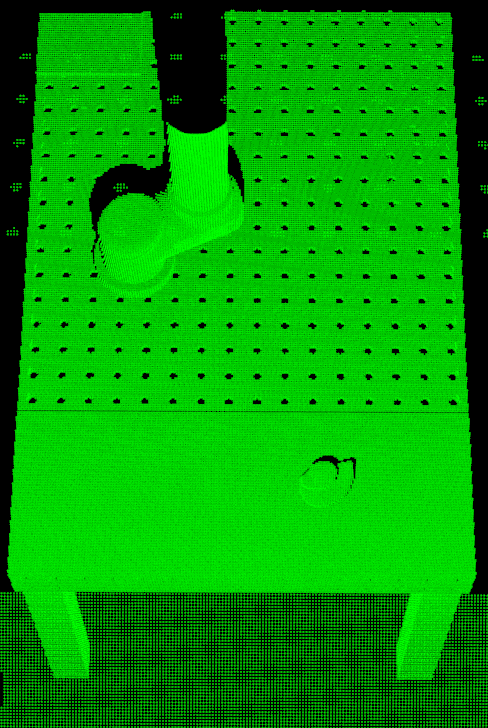
\includegraphics[width=0.15\textwidth]{figures/simulated_depth_sensor/scene_before_preprocessing.png}};
% \node at (-1, -5) {(a) Initial scene};
% \draw[->, dashed] (0.25,-3) -- (1.75,-3);

% % scene after proprocessing
% \node[inner sep=0pt] (vertical) at (3, -3) {
\includegraphics[width=0.15\textwidth]{figures/simulated_depth_sensor/scene_after_preprocessing.png}};
% \node at (3, -5) {(b) Filtered scene};
% \node at (3, -5.5) {with object};
% \draw[->] (4.25,-3) -- (5.75,-3);

% % scene after global alignment
% \node[inner sep=0pt] (vertical) at (7, -3) {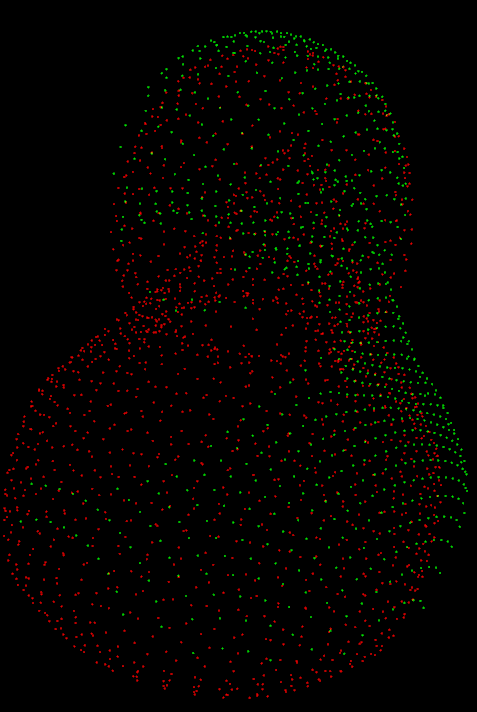
\includegraphics[width=0.15\textwidth]{figures/simulated_depth_sensor/after_global_alignment.png}};
% \node at (7, -5) {(c) After global};
% \node at (7, -5.5) {alignment};
% \draw[->] (8.25,-3) -- (9.75,-3);

% % scene after local alignment
% \node[inner sep=0pt] (vertical) at (11, -3) {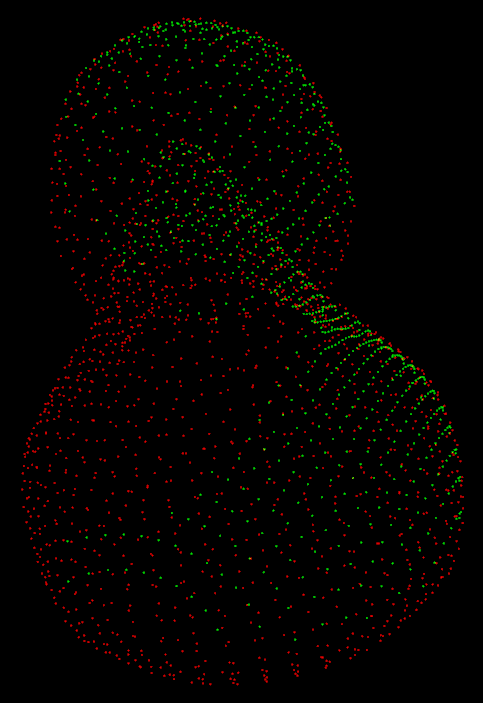
\includegraphics[width=0.15\textwidth]{figures/simulated_depth_sensor/after_local_alignment.png}};
% \node at (11, -5) {(d) After local};
% \node at (11, -5.5) {alignment};
% \draw[->, dashed] (12,-3) -- (12.5,-3);

% \node[cloud] at (13.5,-3) {Pose};

\end{tikzpicture}